\documentclass[12pt,a4paper]{jsarticle}

\usepackage[utf8]{inputenc}     % 文字コードをUTF-8に指定
\usepackage[dvipdfmx]{graphicx} % グラフィクスの利用宣言
\usepackage{multirow}           % 表でのセル結合
\usepackage{dcolumn}            % 表での小数点揃え
\usepackage{amssymb}            % 数学記号などの利用宣言
\usepackage{mathtools}          % 数式の記述を助けるパッケージ
\usepackage{amsmath}            % 数式の記述を助けるパッケージ
\usepackage{siunitx}            % SI単位系の利用宣言
\usepackage{bm}                 % 太字数式文字の利用に関する宣言
\usepackage{float}              % 図表の位置を固定する
\usepackage{url}                % URLの記述を助けるパッケージ
\usepackage{listings}           % ソースコードの記述を助けるパッケージ
\usepackage{jvlisting}          % ソースコードの日本語対応
\usepackage{xcolor}             % 色の指定
\usepackage{tikz}               % 図の描画を助けるパッケージ
\usetikzlibrary{arrows.meta, positioning, shapes, shadows.blur, calc}

\lstset{
	%プログラム言語(複数の言語に対応,C,C++も可)
 	language = {Python},
 	%背景色と透過度
 	backgroundcolor={\color[gray]{.90}},
 	%枠外に行った時の自動改行
 	breaklines = true,
 	%自動改行後のインデント量(デフォルトでは20[pt])	
 	breakindent = 10pt,
 	%標準の書体
 	basicstyle = \ttfamily\scriptsize,
 	%コメントの書体
 	commentstyle = {\itshape \color[cmyk]{1,0.4,1,0}},
 	%関数名等の色の設定
 	classoffset = 0,
 	%キーワード(int, ifなど)の書体
 	keywordstyle = {\bfseries \color[cmyk]{0,1,0,0}},
 	%表示する文字の書体
 	stringstyle = {\ttfamily \color[rgb]{0,0,1}},
 	%枠 "t"は上に線を記載, "T"は上に二重線を記載
	%他オプション:leftline,topline,bottomline,lines,single,shadowbox
 	frame = TBrl,
 	%frameまでの間隔(行番号とプログラムの間)
 	framesep = 5pt,
 	%行番号の位置
 	numbers = left,
	%行番号の間隔
 	stepnumber = 1,
	%行番号の書体
 	numberstyle = \tiny,
	%タブの大きさ
 	tabsize = 2,
 	%キャプションの場所("tb"ならば上下両方に記載)
 	captionpos = t
}

%%%%%%%%%%%%%%%%%%%%%%%%%%%%%%%%%%%%%%%%%%%%%%%%%%%%%%%%%%%%%%%%%%%%%%%%%%%%%%%%%%%%%%%%%%%%%%%%%%%%

\title{臨床意思決定支援のための検索拡張生成 (RAG) システムの提案および実装}
\author{2581008 \quad 井上 裕介}
\date{2025年7月3日}

%%%%%%%%%%%%%%%%%%%%%%%%%%%%%%%%%%%%%%%%%%%%%%%%%%%%%%%%%%%%%%%%%%%%%%%%%%%%%%%%%%%%%%%%%%%%%%%%%%%%

% ここから本体
\begin{document}

\pagenumbering{arabic}           % ページ番号をアラビア数字になおす
\renewcommand{\figurename}{図}    % キャプションをFigureから図にする
\renewcommand{\tablename}{表}     % キャプションをTableから表にする
\numberwithin{equation}{section} % 式番号をセクション毎にリセットする
\maketitle                       % タイトルを出力

%%%%%%%%%%%%%%%%%%%%%%%%%%%%%%%%%%%%%%%%%%%%% ↓ EDIT ↓ %%%%%%%%%%%%%%%%%%%%%%%%%%%%%%%%%%%%%%%%%%%%%

\section{はじめに}
\label{sec:ex1}
\subsection*{(1)}

本レポートは、臨床意思決定支援に特化した検索拡張生成 (RAG) システムの設計、実装、および評価について述べる。
汎用大規模言語モデル (LLM) が、医療のような高リスク領域において、ハルシネーションや古い知識、文脈的根拠の欠如といった重大な限界を抱えていることに着目した。
これらの限界は患者の安全に直接的な脅威となり、最適な医療提供の障害となる。
この課題に対処するため、LLMを「閉じた本の試験」から「開いた本の試験」へと変革するアプローチであるRAGが不可欠であると論じている。
RAGは、ユーザーの質問に対し、外部の信頼できる知識ベース (電子カルテから構築された精選された知識ベース) から関連情報を検索し、それをLLMに提供することで、提示された証拠に基づく応答生成を強制する。
この転換は、ハルシネーションを削減し、最新情報へのアクセスを可能にし、応答の追跡可能性と説明可能性を確保することで、エビデンスに基づく実践のパラダイムにシステムを近づける。
本システムは、実世界の臨床ノートの代理としてMIMIC-IVデータセットを利用し、医学文書のセマンティックな完全性を維持するためのメタデータ拡張チャンキング戦略と、日本語に特化した医療用埋め込みモデルを活用して実装された。
評価はRAGASフレームワークを用いて行われ、臨床情報アクセスを強化するRAGの有効性が示されている。

\section{Retrieval-Augmented Generation}
\label{sec:ex2}

Retrieval-Augmented Generation (RAG) は、ユーザーの質問に対して外部の知識ベースから情報を検索し、それを基に応答を生成する手法である。
RAGは、特に医療のような高リスク領域において、信頼性の高い情報を提供するために重要である。
RAGの基本的な流れは以下の通りである。
\begin{enumerate}
	\item ユーザーの質問を受け取る
	\item 質問に関連する情報を外部の知識ベースから検索する
	\item 検索結果を基に、LLMが応答を生成する
	\item 応答をユーザーに提供する
\end{enumerate}
RAGは、応答からソース文書への直接的な証拠の追跡を可能にし、これは現代医療の礎であるエビデンスに基づく実践 (Evidence-Based Practice) のパラダイムにシステムを近づけるものであるとされている。

\section{システムの構成}
\label{sec:ex3}

\begin{figure}[H]
    \centering
    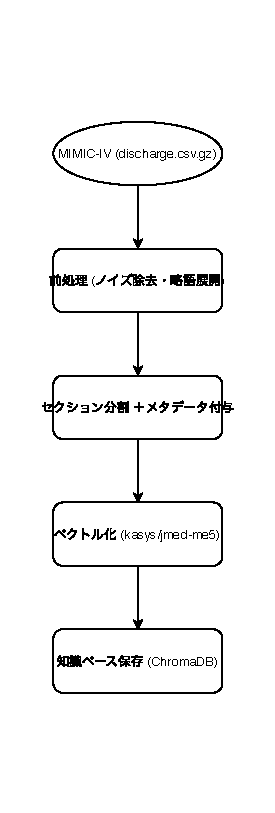
\includegraphics[width=0.8\textwidth]{RAG_Flowchart1.pdf}
    \caption{RAGシステムのアーキテクチャ}
    \label{fig:rag_system_architecture}
\end{figure}

\begin{figure}[H]
    \centering
    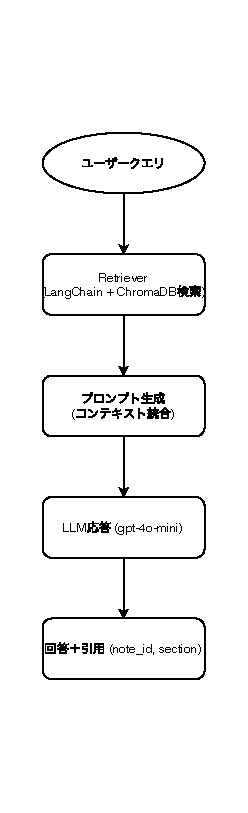
\includegraphics[width=0.8\textwidth]{RAG_Flowchart2.pdf}
    \caption{RAGシステムのアーキテクチャ}
    \label{fig:rag_system_architecture2}
\end{figure}

RAGシステムの中核的なメカニズムは、ユーザーの質問(クエリ)がまず外部の信頼できる知識ベースからの検索ステップを引き起こすことから始まる。
この検索されたコンテキスト(文脈)が、元のプロンプトに「拡張(augment)」されてLLMに提供され、LLMはこの与えられた特定の情報に基づいて応答を生成する。
この構造により、LLMの応答生成は、確率的な推測から提示された証拠に基づく合成へと転換される。
システムの設計においては、実世界の臨床ノートの代理としてMIMIC-IVデータセットが利用された。
医学文書のセマンティックな完全性を維持するため、メタデータで拡張された高度なチャンキング戦略が採用されたアーキテクチャが設計されている。
また、ドメインの関連性を確保するために、日本語に特化した医療用埋め込みモデルを活用している。

\section{実装}
\label{sec:ex4}

ここからは、RAGシステムの実装に関する詳細を述べる。
本RAGシステムの構築と展開には多くの工数を必要とする。
これらの作業は知識ベースの品質に決定的に依存する。
そのため、文書の元の意味構造を保持し、メタデータでそれを豊かにする高度なインジェスチョンパイプラインへの投資が最もレバレッジの効く活動とされた。
本章では、LangChainフレームワークを用いて、前章で設計したデータパイプラインとRAGのコアロジックを実装する具体的なPythonコードと手法について解説する。

\subsection{データパイプラインの設計と実装}
はじめに、データ処理パイプラインは、MIMIC-IV-Noteデータセットのdischarge.csv.gzファイルをロードすることから始まる。
実際のEHRデータに含まれるノイズを処理するため、正規表現などを用いて以下のクリーニングを行う。
\begin{itemize}
	\item 不要な空白や一貫性のないフォーマットの除去
	\item セクションヘッダーの標準化
	\item MIMIC-IVの匿名化処理で生じるアーティファクトの適切な処理
\end{itemize}

\subsection{メタデータの拡張とセクションベースの解析}
次に、セクションベースの解析について述べる。
医療記録のような構造化された文書に対して、単純なチャンキング戦略は不十分である。
文脈を不自然に分断し、検索されるチャンクの有用性を損なう可能性があるためである。
そこで、本プロジェクトではよりインテリジェントなセクション認識型のアプローチを実装する。
まず退院サマリーを構成セクションに解析することである。
MIMICノートに関する研究によれば、これらは半構造化されたフォーマットを持ち、共通のヘッダーが存在する。
正規表現を用いて、以下のようなヘッダーを特定し、その配下のテキストを抽出する。
\begin{itemize}
	\item Chief Complaint (主訴)
	\item History of Present Illness (現病歴)
	\item Past Medical History (既往歴)
	\item Allergies (アレルギー)
	\item Medications on Admission (入院時処方薬)
	\item Physical Exam (身体所見)
	\item Brief Hospital Course (入院経過概要)
	\item Discharge Diagnosis (退院時診断)
	\item Discharge Medications (退院時処方薬)
\end{itemize}
このセクションベースの解析により、各セクションが独立したコンテキストとして扱われ、検索精度が向上する。

\subsection{メタデータの定義と埋め込みモデルの選定}
次に、メタデータの定義と埋め込みモデルの選定について述べる。
メタデータは、各セクションのコンテキストを豊かにし、検索精度を向上させるための重要な要素である。
最終的にChromaDBの各ベクトルと共に格納される、リッチなメタデータ構造を以下のように定義する。
\lstset{language={Python}}
\begin{lstlisting}[language=Python, label=lst:JSON, caption=提案スキーマ (JSON形式)]
{
  "source_file": "discharge_12345.txt",
  "note_id": "note_xyz",
  "patient_id": "p_001",
  "admission_id": "adm_001",
  "note_type": "Discharge Summary",
  "section_header": "Discharge Medications",
  "chunk_id": "note_xyz_chunk_5",
  "snomed_ct_codes": ["73211009", "386661006"],
  "icd10_codes": ["E11.9", "I10"]
}
\end{lstlisting}
このメタデータは単なる記述情報ではなく、検索精度を向上させるための強力なフィルタリングツールとして機能する。
このスキーマは、強力なハイブリッド検索戦略を可能にする。
例えば、臨床医が「入院ID adm\_001 の患者の退院時処方薬は何でしたか?」と質問した場合、システムはまずベクトル空間全体からadmission\_id == "adm\_001" かつ section\_header == "Discharge Medications" であるチャンクをフィルタリングし、その非常に小さく関連性の高いサブセット内でクエリのセマンティック検索を実行できる。
これは、データベース全体に対するブルートフォース検索よりもはるかに効率的かつ正確である。
また、SNOMED-CTやICD-10コードをメタデータに含めることで、コードベースの検索や、オントロジーを利用したより高度なクエリへの拡張性も確保できる。

\subsection{埋め込みモデルのロード}
まず、選定した日本語医療用埋め込みモデルkasys/jmed-me5-v0.1をロードする。
このモデルは最適な性能を発揮するために、クエリと文書で異なるプレフィックスを要求するため、その設定も行う。
\lstset{language={Python}}
\begin{lstlisting}[language=Python, label=lst:loadmodel, caption=埋め込みモデルのロード]
from langchain_huggingface import HuggingFaceEmbeddings

# モデル名とプレフィックス設定
model_name = "kasys/jmed-me5-v0.1"
model_kwargs = {'device': 'cpu'} # or 'cuda'
encode_kwargs = {'normalize_embeddings': True}

# プレフィックスはモデルの性能に重要
# クエリ用と文書用で異なる設定を行う
hf_embeddings = HuggingFaceEmbeddings(
    model_name=model_name,
    model_kwargs=model_kwargs,
    encode_kwargs=encode_kwargs,
    query_instruction="query: ", # クエリ用のプレフィックス
    embed_instruction="passage: " # 文書用のプレフィックス
)
\end{lstlisting}

\subsection{ChromaDBの初期化とインデックス作成}
次に、作成したベクトルを永続的に保存するため、ChromaDBクライアントを初期化し、前処理済みの文書をインデックスに追加する。
ID生成ロジックは、再登録時に重複を防ぎ、更新を可能にするために重要である。
\lstset{language={Python}}
\begin{lstlisting}[language=Python, label=lst:chroma_init, caption=ChromaDBの初期化とインデックス作成]
import chromadb
from langchain_chroma import Chroma
import os

# 永続化ディレクトリを指定
persist_directory = "./chromadb_store"
collection_name = "medical_notes_jp"

# ChromaDBクライアントを初期化
client = chromadb.PersistentClient(path=persist_directory)

# LangChainのChromaラッパーを初期化
vector_store = Chroma(
    client=client,
    collection_name=collection_name,
    embedding_function=hf_embeddings,
)

# preprocessed_documentsは第4章で作成したDocumentオブジェクトのリスト
# 各Documentはpage_contentとmetadataを持つ

# ユニークIDのリストを作成
# 例: metadata['source']とmetadata['start_index']を組み合わせる
ids = [
    f"{os.path.splitext(doc.metadata['source'])}_{doc.metadata['start_index']}"
    for doc in preprocessed_documents
]

# ドキュメントをChromaDBに追加(UPSERT動作)
vector_store.add_documents(documents=preprocessed_documents, ids=ids)
\end{lstlisting}

\subsection{LangChainのリトリーバの設定}
作成したvector\_storeをLangChainのリトリーバとして設定する。
ここでは、先ほど設計したメタデータによるフィルタリングを活用した検索も可能である。
\lstset{language={Python}}
\begin{lstlisting}[language=Python, label=lst:retriever, caption=LangChainのリトリーバの設定]
retriever = vector_store.as_retriever(
    search_type="similarity",
    search_kwargs={'k': 5} # 上位5件のチャンクを検索
)

# メタデータフィルタリングを用いたリトリーバの例
# 例:特定の患者の「退院時処方薬」セクションのみを検索対象とする
metadata_filtered_retriever = vector_store.as_retriever(
    search_type="similarity",
    search_kwargs={
        'k': 5,
        'filter': {
            "patient_id": "p_001",
            "section_header": "Discharge Medications"
        }
    }
)
\end{lstlisting}

\subsection{RAGシステムの実装}
LangChain Expression Language (LCEL) を用いて、検索から生成までの一連の処理をパイプとして結合する。
RunnablePassthroughは、元の質問をチェーンの後のステップに渡すために使用される。
\lstset{language={Python}}
\begin{lstlisting}[language=Python, label=lst:rag_chain, caption=RAGチェーンの構築]
from langchain_core.runnables import RunnablePassthrough
from langchain_core.output_parsers import StrOutputParser
from langchain_openai import ChatOpenAI

# LLMの初期化(第3章で選定)
llm = ChatOpenAI(model_name="gpt-4o-mini", temperature=0)

# プロンプトテンプレート(次節で詳述)
prompt = hub.pull("rlm/rag-prompt") # またはカスタムプロンプト

def format_docs(docs):
    return "\n\n".join(doc.page_content for doc in docs)

# RAGチェーンの定義
rag_chain = (
    {"context": retriever | format_docs, "question": RunnablePassthrough()}
| prompt
| llm
| StrOutputParser()
)

# チェーンの実行
question = "患者p_001の退院時処方薬について教えてください。"
response = rag_chain.invoke(question)
print(response)
\end{lstlisting}

\subsection{プロンプトテンプレートの設計}
LLMを安全かつ正確に導くためには、精巧に設計されたプロンプトが不可欠である。
以下に、本プロジェクトで採用するプロンプトテンプレートとその設計思想を示す。

\lstset{language={Python}}
\begin{lstlisting}[language=Python, label=lst:rag_prompt, caption=RAGプロンプトテンプレート]
"あなたは高度なスキルを持つ臨床意思決定支援アシスタントです。あなたの目的は、提供された患者の電子カルテのコンテキストに「のみ」基づいて、質問に正確に回答することです。あなた自身の内部知識は一切使用しないでください。"
"もし提供されたコンテキストに質問に答えるために必要な情報が含まれていない場合は、必ず「提供されたコンテキストには、この質問に回答するための十分な情報が含まれていません。」と回答してください。存在しない情報を推測したり、推論したりしようとしないでください。"

"コンテキスト:"

{context}

"上記のコンテキストに基づき、以下の質問に回答してください。回答に使用する各情報について、具体的なソース文書とセクションを引用してください。"

"質問: {question}"

"回答:"
\end{lstlisting}


%%%%%%%%%%%%%%%%%%%%%%%%%%%%%%%%%%%%%%%%%%%%% ↑ EDIT ↑ %%%%%%%%%%%%%%%%%%%%%%%%%%%%%%%%%%%%%%%%%%%%%


\end{document}